\documentclass[oneside,final]{article}
\usepackage[utf8]{inputenc}
\usepackage[russian]{babel}
\usepackage{vmargin}
\usepackage{mathtext}
\usepackage{graphicx}
\usepackage{amsfonts}
\usepackage{amsmath}
\usepackage{float}
\usepackage[unicode, pdftex]{hyperref}
\DeclareGraphicsExtensions{.pdf,.png,.jpg}
\graphicspath{{images/}}
\setpapersize{A4}
\addto\captionsrussian{\def\refname{Литература`}}
\usepackage{indentfirst}
\begin{document}
	\begin{titlepage}
		\newpage 
		\begin{center}
			{\bfseries Санкт-Петербургский политехнический университет
			Петра Великого \\
			Институт прикладной математики и механики
				Кафедра «Прикладная математика»\\}  
			\vfill
			\vfill
			\normalsize{Отчет по лабораторной работе 9\\
					по дисциплине\\
				«Математическая статистика»\\}   
			\vfill		                    
		\end{center}
		\begin{flushright}
		\begin{minipage}{.45\textwidth}
			\normalsize{Выполнил студент:\\
			Файзрахманов А. Р. \\
			группа: 5030102/90201}
			\break\hfill\break
			\\
			\normalsize{Проверил:\\
			к.ф.-м.н., доцент\\
			Баженов Александр Николаевич} 
		
\end{minipage}
		\end{flushright}
		\begin{center}
			\vfill
			\normalsize{Санкт-Петербург, 2022}
		\end{center}
	\end{titlepage}

	\tableofcontents
	\newpage
	\listoffigures
	\newpage
	\section{Постановка задачи}
\begin{enumerate}

	\item {Сгенерировать двумерные выборки размерами 20, 60, 100 для нормального двумерного распределения $N(x, y, 0, 0, 1, 1, \rho)$.\\ 	Коэффициент корреляции $\rho$ взять равным 0, 0.5, 0.9.\\ Каждая выборка генерируется 1000 раз и для неё вычисляются: среднее значение, среднее значение квадрата и дисперсия коэффициентов корреляции Пирсона, Спирмена и квадрантного коэффициента корреляции.\\Повторить все вычисления для смеси нормальных распределений:\\$$f(x, y) = 0.9N(x, y, 0, 0, 1, 1, 0.9) + 0.1N(x, y, 0, 0, 10, 10, -0.9).$$\\Изобразить 		сгенерированные точки на плоскости и нарисовать эллипс равновероятности.}

	\item {Найти оценки коэффициентов линейной регресии $y_i = a + bx_i + e_i$, используя 20 точек на отрезке $[-1.8; 2]$ с равномерным шагом равным 0.2. Ошибку $e_i$ считать нормально распределенной с параметрами $(0, 1)$. В качестве эталонной зависимости взять  $y_i = 2 + 2x_i + e_i$. При построении оценок коэффициентов использовать два критерия: критерий наименьших квадратов и критерий наименьших модулей. Проделать то же самое для выборки, у которой в значении $y_1$ и $y_{20}$ вносятся возмущения 10 и -10}

	\item {Сгенерировать выборку объёмом 100 элементов для нормального распределения $N(x, 0, 1)$. По сгенерированной выборке оценить параметры $\mu$ и $\sigma$ нормального закона методом максимального правдоподобия. В качестве основной гипотезы $H_0$ будем считать, что сгенерированное распределение имеет вид $N(x, \hat{\mu}, \hat{\sigma})$. Проверить основную гипотезу, используя критерий согласия $\chi^2$. В качестве уровня значимости взять $\alpha = 0.05$. Привести таблицу вычислений $\chi^2$.\\Исследовать точность (чувствительность) критерия $\chi^2$ - сгенерировать выборки равномерного распределения и распределения Лапласа малого объема (например, 20 элементов). Проверить их на нормальность.}

	\item {Для двух выборок размерами 20 и 100 элементов, сгенерированных согласно нормальному закону $N(x, 0, 1)$, для параметров положения и масштаба построить асимптотически нормальные интервальные оценки на основе точечных оценок метода максимального правдоподобия и классические интервальные оценки на основе статистик $\chi^2$ и Стьюдента. В качестве параметра надёжности взять $\gamma = 0.95$. }

\end{enumerate}
\newpage

\section{Теория}
\subsection {Рассматриваемые распределения}
	Плотности:
	\begin {itemize}
		\item {Нормальное распределение\\ \begin{equation}N(x, 0, 1) = \frac{1}{\sqrt{2\pi}}e^{-\frac{x^2}{2}}\end{equation}}
		\item {Распределение Коши\\ \begin{equation}C(x, 0, 1) = \frac{1}{\pi}\frac{1}{x^2+1}\end{equation}}
		\item {Распределение Лапласа\\ \begin{equation}L(x, 0, \frac{1}{\sqrt{2}}) = \frac{1}{\sqrt{2}}e^{-\sqrt{2}|x|}\end{equation}}
		\item {Распределение Пуассона\\ \begin{equation}P(k, 10) = \frac{10^k}{k!}e^{-10}\end{equation}}
		\item {Равномерное распределение\\ \begin{equation}U(x, -\sqrt{3}, \sqrt{3}) = 
										\begin{cases}
											\frac{1}{2\sqrt{3}} \text{ при } |x| \leq \sqrt{3} \\
											0  \text{ при } |x| > \sqrt{3}
										\end{cases}\end{equation}}
	\end {itemize}

\subsection {Гистограмма}
	\subsubsection {Построение гистограммы}
		Множество значений, которое может принимать элемент выборки, разбивается на несколько интервалов. Чаще всего эти интервалы берут одинаковыми, но это не является строгим требованием. Эти интервалы откладываются на горизонтальной оси, затем над каждым рисуется прямоугольник. Если все интервалы были одинаковыми, то высота каждого прямоугольника пропорциональна числу элементов выборки, попадающих в соответствующий интервал. Если интервалы разные, то высота прямоугольника выбирается таким образом, чтобы его площадь была пропорциональна числу элементов выборки, которые попали в этот интервал [1].
	
	\subsubsection {Вариационный ряд}
		Вариационным ряд - последовательность элементов выборки, расположенных в неубывающем порядке. Одинаковые элементы повторяются [2, с. 409].

\subsection {Выборочные чиловые характеристики}
	\subsubsection {Характеристики положения}
		\begin{itemize}
			\item {Выборочное среднее\\ \begin{equation}\overline{x} = \frac{1}{n}\sum_{i=1}^{n}x_i\end{equation}}

			\item {Выборочная медиана\\ \begin{equation}med\ x = 
									\begin{cases}
										x_{(l+1)} \text{ при } n = 2l + 1 \\
										\frac{x_{(l)} + x_{(l+1)}}{2} \text{ при } n=2l
									\end{cases}\end{equation}}

			\item {Полусумма экстремальных выборочных элементов \\ \begin{equation}z_R =  \frac{x_{(1)}+x_{(n)}}{2}\end{equation}}

			\item {Полусумма квартилей\\
			Выборочная квартиль $z_p$ порядка $p$ определяется формулой \\ 
			\begin{equation}z_p = \begin{cases} x_{([np]+1)} \text{ при } np \text{ дробном,} \\ x_{(np)} \text{ при } np \text{ целом.} \end{cases}\end{equation}\\
			Полусумма квартилей\\
				\begin{equation}z_Q = \frac{z_{1/4} + z_{4/4}}{2}\end{equation}}

			\item {Усечённое среднее \\ \begin{equation}z_{tr} = \frac{1}{n-2r}\sum_{i=r+1}^{n-r}x_{(i)},\ r\approx \frac{n}{4}\end{equation}}
		\end{itemize}
	
	\subsubsection {Характеристики рассеяния}
		Выборочная дисперсия \\
		\begin{equation}D = \frac{1}{n}\sum_{i=1}^{n}(x_i-\overline{x})^2\end{equation}

\subsection {Боксплот Тьюки}
	\subsubsection {Построение}
		Границами ящика – первый и третий квартили, линия в середине ящика — медиана. Концы усов — края статистически значимой выборки (без выбросов). Длина «усов»:\\
			\begin{equation}X_1 = Q_1 - \frac{3}{2}(Q_3 - Q_1),\ X_2 = Q_3 + \frac{3}{2}(Q_3 - Q_1)\end{equation} \\ 
		где $X_1$ - нижняя граница уса, $X_2$ - верхняя граница уса, $Q_1$ - первый квартиль, $Q_3$ - третий квартиль.\\
			Данные, выходящие за границы усов (выбросы), отображаются на графике
в виде маленьких кружков [3].

	\subsubsection {Теоретическая вероятность выбросов}
		Можно вычислить теоретические первый и третий квартили распределений - $Q_1^T$ и $Q_3^T$. По ф-ле (15) – теоретические нижнюю и верхнюю границы уса $X_1^T$ и $X_2^T$.  Выбросы – величины $x$:\\
	\begin{equation}
		\left[
			\begin{gathered}
				x < X_1^T \\
				x > X_2^T
			\end{gathered}
		\right.
	 \end{equation}
	Для теоретиеских распределений:\\
	\begin{itemize}
		\item {Для непрерывных распределений\\ 
				\begin{equation} P_B^T = P(x < X_2^T) + P(x > X_2^T) = F(X_1^T) + (1 - F(X_2^T)) \end{equation}}
		
		\item {Для дискретных распределений\\
				\begin{equation} P_B^T = P(x < X_2^T) + P(x > X_2^T) = (F(X_1^T) - P(x = X_1^T)) + (1 - F(X_2^T)) \end{equation}}
	\end{itemize}


\subsection {Эмпирическая функция распределения}
	\subsubsection {Статистический ряд}
		Статистический ряд - последовательность упорядоченных по возрастанию различных элементов выборки $z_1, z_2, ..., z_k$ и и частот, с которыми эти элементы встречаются в выборке $n_1, n_2, ..., n_k$. 

	\subsubsection {Эмпирическая функция распределения}
		Эмпирическая функция распределения сопоставляет числу $x$ относительную частоту события $X<x$, полученную по данной выборке:\\
	\begin{equation} F_n^* = P^*(X<x)\end{equation}

	\subsubsection {Нахождение э. ф. р.}
		Для получения относительной частоты $P^*(X<x)$ просуммируем в статистическом ряде, построенном по данной выборке, все частоты $n_i$, для которых элементы $z_i$ статистического ряда меньше $x$. Тогда $P^*(X<x) = \frac{1}{n} \sum_{z_i<x}n_i$. Получаем\\
	\begin{equation} F^*(x) = \frac{1}{n}\sum_{z_i<x} n_i\end{equation}

\subsection {Оценки плотности вероятности}
	\subsection {Определение}
		Оценкой плотности вероятности $f(x)$ называется функция $\hat{f}(x)$, построенная на основе выборки, приближённо равная $f(x)$\\
		\begin{equation} \hat{f}(x) \approx f(x) \end{equation}

	\subsection {Ядерные оценки}
		Представим оценку в виде суммы с числом слагаемых, равным объёму выборки: \\
		\begin{equation} \hat{f}_n(x) = \frac{1}{nh_n}\sum_{i=1}^{n}K(\frac{x-x_i}{h_n})\end{equation}
		Здесь функция $K(u)$называемая ядерной (ядром), непрерывна и является плотностью вероятности, $x_1, x_2, ..., x_n$ - элементы выборки, $\{h_n\}$ - любая последовательность положительных чисел, обладающая свойствами\\
	\begin{equation} h_n \underset{n\to \infty}{\longrightarrow} 0;\ \ \ \frac{h_n}{n^{-1}} \underset{n \to \infty}{\longrightarrow} \infty \end{equation}\\
	Гауссово (нормальное) ядро [4, с. 38]\\
	\begin{equation} K(u) = \frac{1}{\sqrt{2\pi}}e^{-\frac{u^2}{2}}\end{equation}\\
	Правило Сильвермана [4, с. 44]\\
	\begin{equation} h_n = 1.06\hat{\sigma}n^{-1/5}\end{equation}\\
	где $\hat{\sigma}$ - выборочное стандартное отклонение.

\newpage

\section{Реализация}
Лабораторная работа выполнена на языке программирования Python с помощью библиотек numpy, matplotlib, scipy, statsmodels. Отчет написан в среде разработки TexWorks с помощью pdfLaTeX

\section{Результаты}
\begin{figure}[H]
	\center{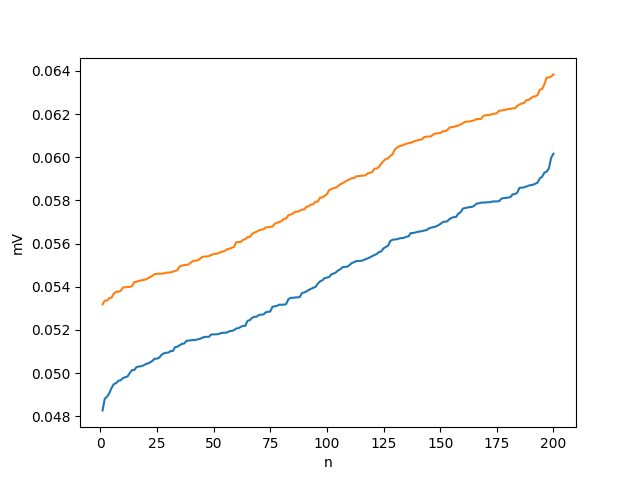
\includegraphics[width=0.5\linewidth]{images/data.png}}
	\caption{Результаты измерений величины токов.}
	\label{ris:image2}
\end{figure}

\begin{figure}[H]
	\center{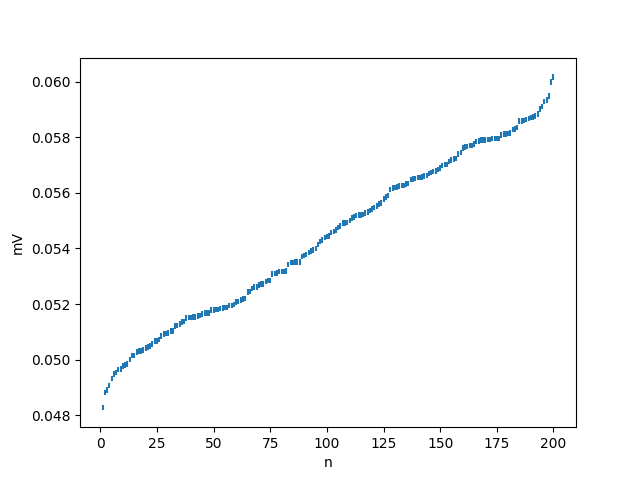
\includegraphics[width=0.5\linewidth]{images/data_and_intervals1.png}}
	\caption{Интервальное представление данных для выборки 1.}
	\label{ris:image2}
\end{figure}

\begin{figure}[H]
	\center{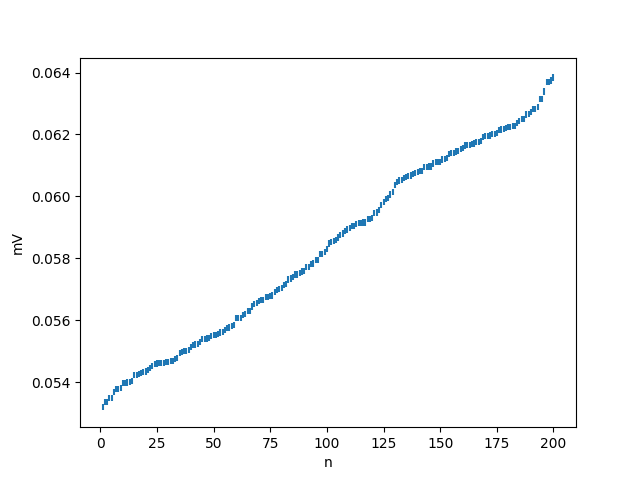
\includegraphics[width=0.5\linewidth]{images/data_and_intervals2.png}}
	\caption{Интервальное представление данных для выборки 2.}
	\label{ris:image2}
\end{figure}

\begin{figure}[H]
	\center{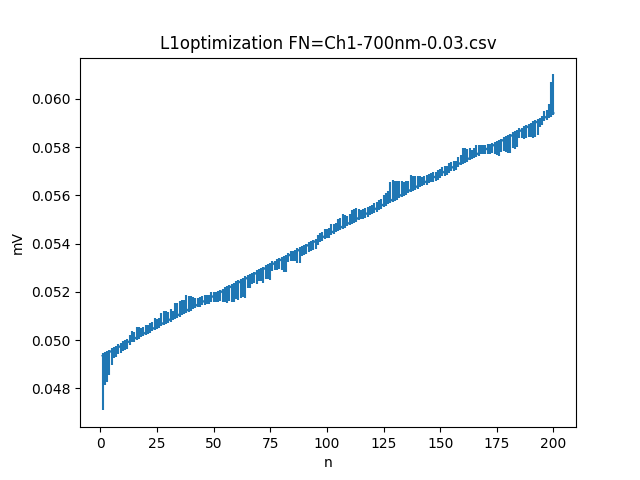
\includegraphics[width=0.5\linewidth]{images/di1.png}}
	\caption{Линейная модель дрейфа данных из выборки 1.}
	\label{ris:image1}
\end{figure}

\begin{figure}[H]
	\center{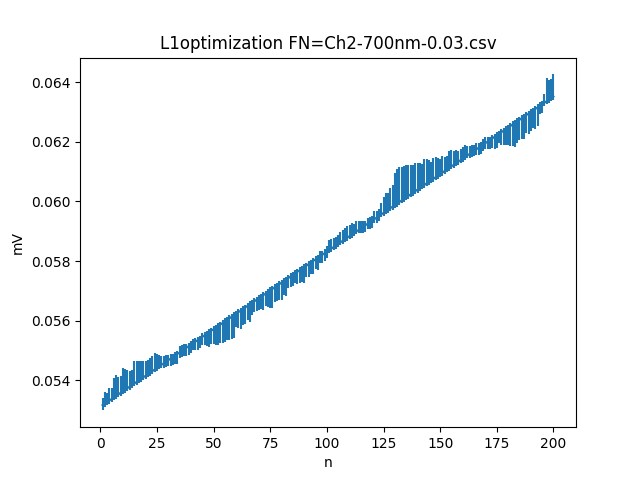
\includegraphics[width=0.5\linewidth]{images/di2.png}}
	\caption{Линейная модель дрейфа данных из выборки 2.}
	\label{ris:image1}
\end{figure}

\begin{figure}[H]
	\center{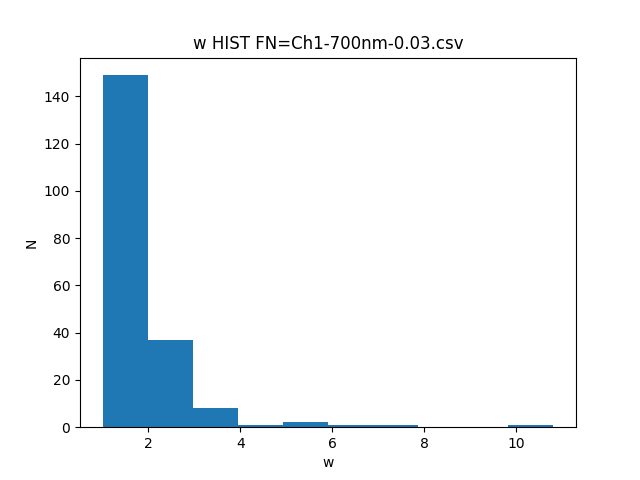
\includegraphics[width=0.5\linewidth]{images/hist1.png}}
	\caption{Гистограмма значений множителей коррекции $w$ из выборки 1.}
	\label{ris:hist1}
\end{figure}

\begin{figure}[H]
	\center{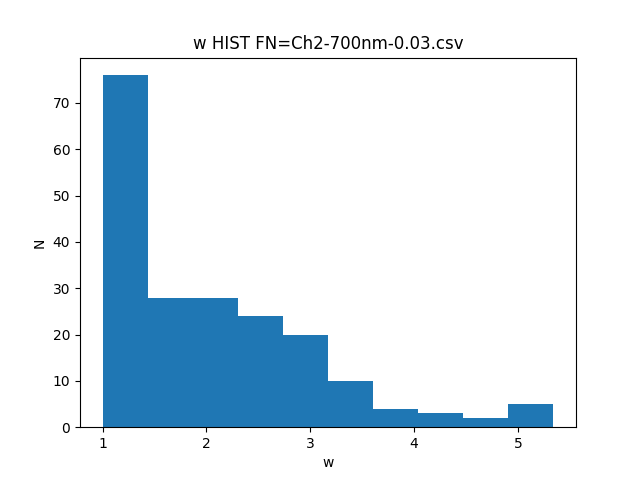
\includegraphics[width=0.5\linewidth]{images/hist2.png}}
	\caption{Гистограмма значений множителей коррекции $w$ из выборки 2.}
	\label{ris:hist2}
\end{figure}

\begin{figure}[H]
	\center{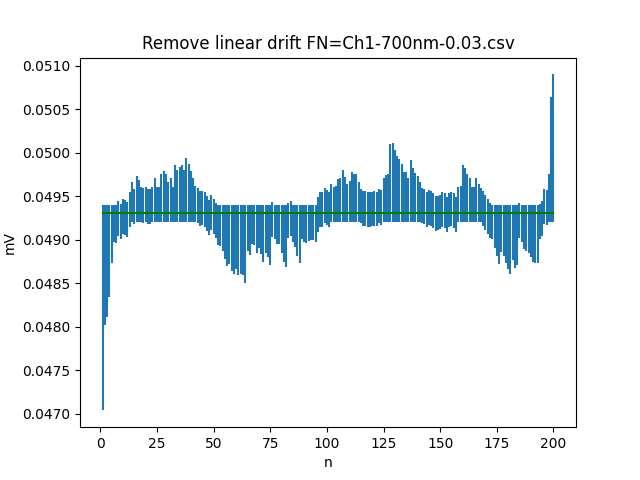
\includegraphics[width=0.5\linewidth]{images/interval_new1.png}}
	\caption{Скорректированная модель данных из выборки 1.}
	\label{ris:hist2}
\end{figure}

\begin{figure}[H]
	\center{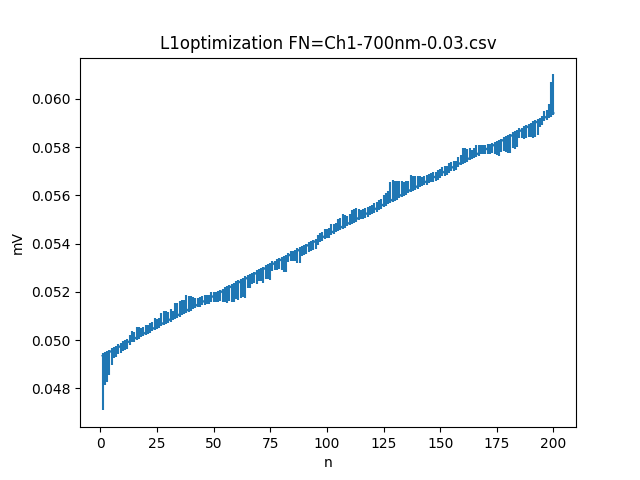
\includegraphics[width=0.5\linewidth]{images/di1.png}}
	\caption{Линейная модель дрейфа данных из выборки 1.}
	\label{ris:image1}
\end{figure}

\begin{figure}[H]
	\center{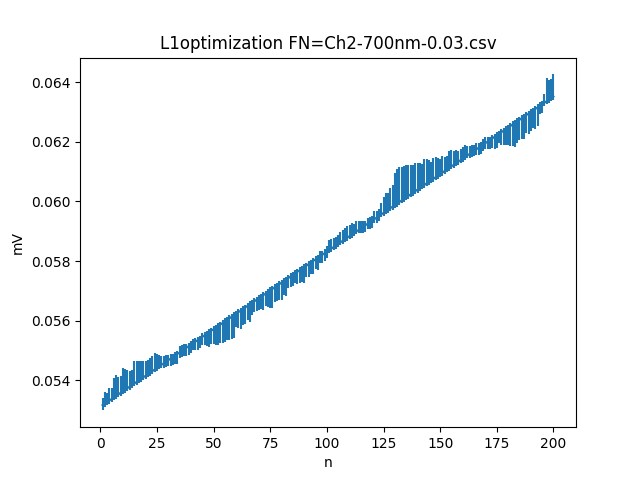
\includegraphics[width=0.5\linewidth]{images/di2.png}}
	\caption{Линейная модель дрейфа данных из выборки 2.}
	\label{ris:image1}
\end{figure}

\begin{figure}[H]
	\center{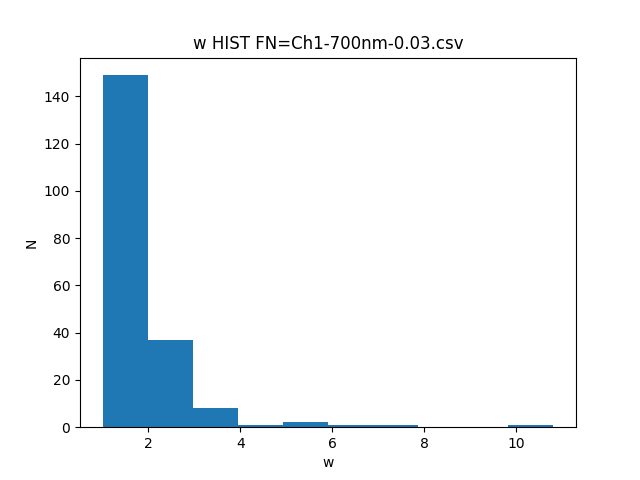
\includegraphics[width=0.5\linewidth]{images/hist1.png}}
	\caption{Гистограмма значений множителей коррекции $w$ из выборки 1.}
	\label{ris:hist1}
\end{figure}

\begin{figure}[H]
	\center{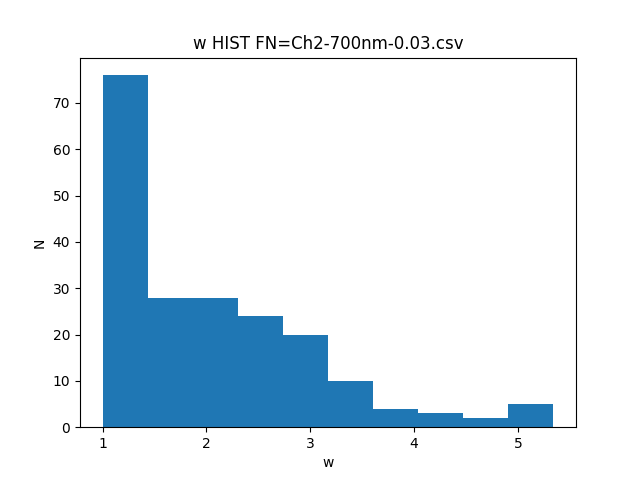
\includegraphics[width=0.5\linewidth]{images/hist2.png}}
	\caption{Гистограмма значений множителей коррекции $w$ из выборки 2.}
	\label{ris:hist2}
\end{figure}

\begin{figure}[H]
	\center{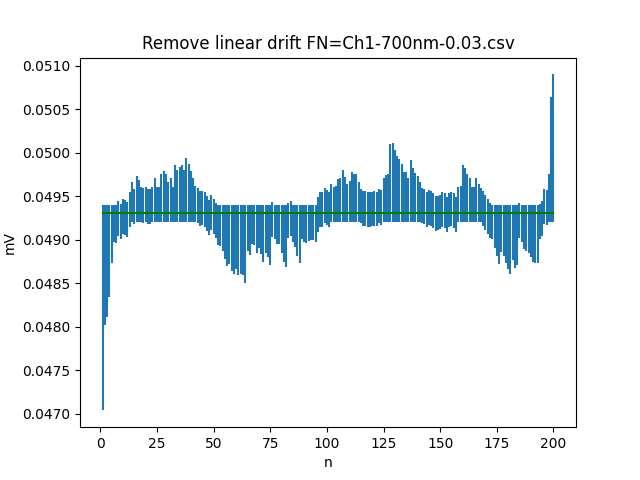
\includegraphics[width=0.5\linewidth]{images/interval_new1.png}}
	\caption{Скорректированная модель данных из выборки 1.}
	\label{ris:hist2}
\end{figure}

\begin{figure}[H]
	\center{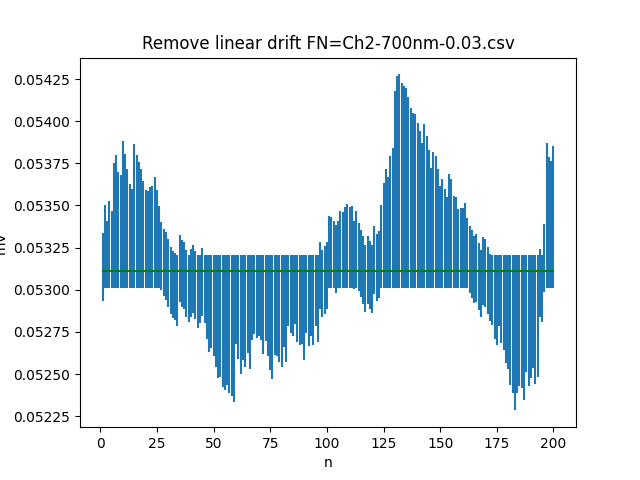
\includegraphics[width=0.5\linewidth]{images/interval_new2.png}}
	\caption{Скорректированная модель данных из выборки 2.}
	\label{ris:hist2}
\end{figure}

\begin{figure}[H]
	\center{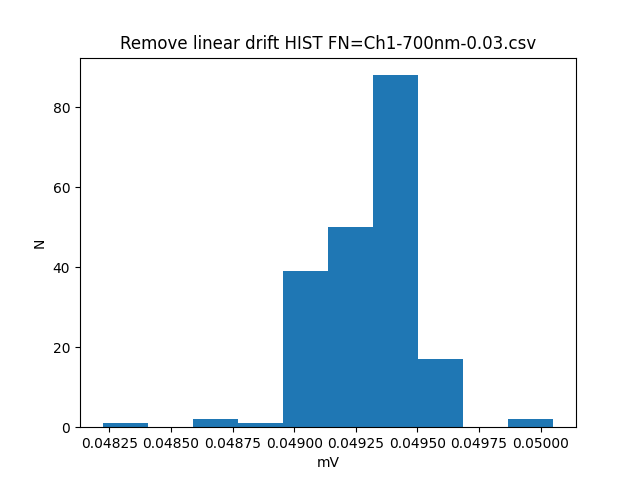
\includegraphics[width=0.5\linewidth]{images/hist_interval1.png}}
	\caption{Гистограмма скорректированной модели данных из выборки 1.}
	\label{ris:hist2}
\end{figure}

\begin{figure}[H]
	\center{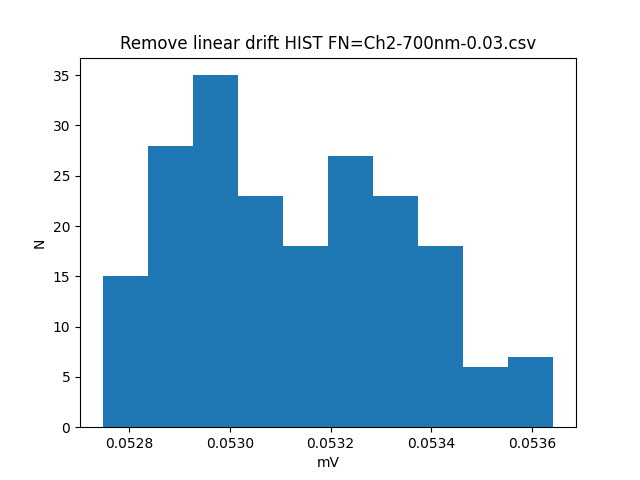
\includegraphics[width=0.5\linewidth]{images/hist_interval2.png}}
	\caption{Гистограмма скорректированной модели данных из выборки 2.}
	\label{ris:hist2}
\end{figure}

\begin{figure}[H]
	\center{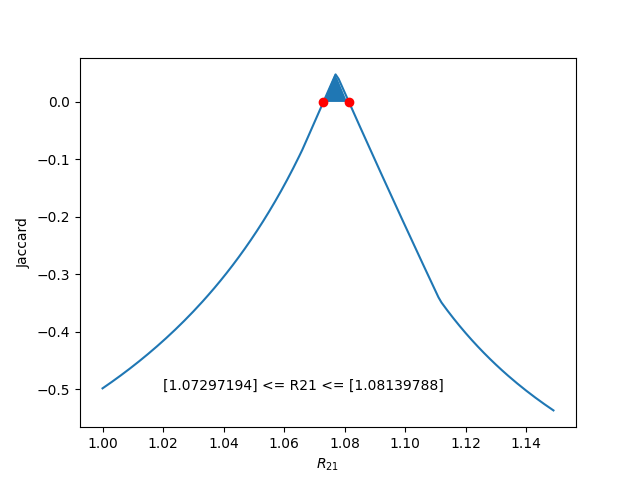
\includegraphics[width=0.5\linewidth]{images/jakkar.png}}
	\caption{Зависимость коэффициента Жаккара от $R_{21}$}
	\label{ris:hist2}
\end{figure}

\begin{figure}[H]
	\center{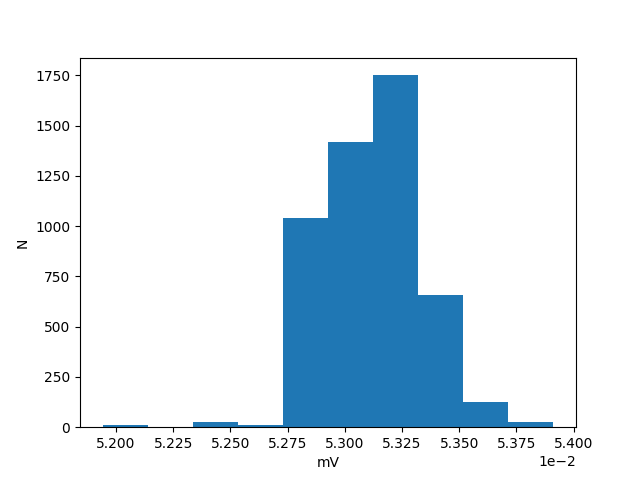
\includegraphics[width=0.5\linewidth]{images/jakkar_combined_hist.png}}
	\caption{Гистограмма объединенной выборки при $R_{21}$}
	\label{ris:hist2}
\end{figure}

\newpage

\section{Обсуждение}
\subsection{Гистограмма и график плотности распределения}
По результатам проделанной работы можем сделать вывод о том, что чем больше выборка для каждого из распределений, тем ближе ее гистограмма к графику плотности вероятности того закона, по которому распределены величины сгенерированной выборки. Чем меньше выборка, тем менее она показательна - тем хуже по ней определяется характер распределения величины.


Также можно заметить, что максимумы гистограмм и плотностей распределения почти нигде не совпали. Также наблюдаются всплески гистограмм, что наиболее хорошо прослеживается на распределении Коши.

\subsection{Характеристики положения и рассеяния}
Исходя из данных, приведенных в таблицах, можно судить о том, что дисперсия характеристик рассеяния для распределения Коши является некой аномалией: значения слишком большие даже при увеличении размера выборки - понятно, что это результат выбросов, которые мы могли наблюдать в результатах предыдущего задания.

\subsection{Доля и теоретическая вероятность выбросов}
По данным, приведенным в таблице, можно сказать, что чем больше выборка, тем ближе доля выбросов будет к теоретической оценке. Снова доля выбросов для распределения Коши значительно выше, чем для остальных распределений. Равномерное распределение же в точности повторяет теоретическую оценку - выбросов мы не получали. 


Боксплоты Тьюки действительно позволяют более наглядно и с меньшими усилиями оценивать важные характеристики распределений. Так, исходя из полученных рисунков, наглядно видно то, что мы довольно трудоёмко анализировали в предыдущих частях.

\subsection{Эмпирическая функция и ядерные оценки плотности распределения}
Можем наблюдать на иллюстрациях с э. ф. р., что ступенчатая эмпирическая функция распределения тем лучше приближает функцию распределения реальной выборки, чем мощнее эта выборка. Заметим так же, что для распределения Пуассона и равномерного распределения отклонение функций друг от друга наибольшее.


Рисунки, посвященные ядерным оценкам, иллюстрируют сближение ядерной оценки и функции плотности вероятности для всех $h$ с ростом размера выборки. Для распределения Пуассона наиболее ярко видно, как сглаживает отклонения увеличение параметра сглаживания $h$.


В зависимости от особенностей распределений для их описания лучше подходят разные параметры $h$ в ядерной оценке: для равномерного распределения и распределения Пуассона лучше подойдет параметр $h = 2h_n$ , для распределения Лапласа - $h = h_n /2$, а для нормального и Коши - $h = h_n$ . Такие значения дают вид ядерной оценки наиболее близкий к плотности, характерной данным распределениям.


Также можно увидеть, что чем больше коэффициент при параметре сглаживания $\hat{h_n}$ , тем меньше изменений знака производной у аппроксимирующей функции, вплоть до того, что при $h = 2h_n$ функция становится унимодальной на рассматриваемом промежутке. Также видно, что при $h = 2h_n$ по полученным приближениям становится сложно сказать плотность вероятности какого распределения они должны повторять, так как они очень похожи между собой.
\newpage

\addcontentsline{toc}{section}{Литература}

\begin{thebibliography}{}
    \bibitem{litlink1} М.З. Шварц. Данные технологических испытаний оборудования для калибровки фотоприемников солнечного излучения. 2022
    \bibitem{litlink2} А.Н. Баженов, С.И. Жилин, С.И. Кумков, С.П. Шарый. Обработка и анализ данных с интервальной неопределенностью. 2022
    \bibitem{litlink3} А.Н. Баженов. Введение в анализ данных с интервальной неопределенностью. 2022
    \bibitem{litlink4} Коэффициент Жаккара \url{https://en.wikipedia.org/wiki/Jaccard\_index}
Jaccard P. Distribution de la flore alpine dans le Bassin des Dranses et dans quelques
regions voisines // Bull. Soc. Vaudoise sci. Natur. 1901. V. 37. Bd. 140. S. 241-272.

    \bibitem{litlink5} С.И. Жилин. Примеры анализа интервальныз данных в Octave \url{https://github.com/szhilin/octave-interval-examples}
\end{thebibliography}

	

\end{document}